\chapter{データベースの異状}\label{chap:anomaly}

\ref{chap:sql-part1}章で例として用いた「商品」テーブルは，データに誤りがないことを前提にしていました．
データベース内のデータが正しく保たれているからこそ，SQLによる正確なデータ分析が可能になり，データベースに接続するアプリケーションも矛盾なく動作します．

\ref{chap:relational-data-model}章で説明したように，関係データモデルにはデータを正しく保つため様々な制約が備わっています．
例えば，前章の「商品」テーブルであれば，「価格は整数でなければならない」というドメイン制約や「商品IDは同じ値を持つことができない」というキー制約を定義することができます．
ドメイン制約やキー制約を定義すれば，RDBMSはデータの登録，更新が行われる際，違反するデータが登録されないよう自動でチェックしてくれます．

ところが，これら制約をテーブルに定義すれば問題なし，というわけにはいかないのです．
こうした制約を設定したとしても，現実のデータベースには誤ったデータが混入していることが多々あります．
ドメイン制約やキー制約は，与えられた関係スキーマに対して，登録されるデータが満たすべきルールを定義するものです．
そのため，テーブルの構造（関係を構成する属性集合）そのもの，つまり関係スキーマが正しく設計されていないと，データベースが冗長になったり，データベース内のレコード間で矛盾が発生したりすることがあります．

関係スキーマが望ましくない構造を持つことによって，関係データベース内に生じる矛盾や不整合を\strong{異状（anomaly）}と呼びます\cite{Codd1970, Codd1972}．
関係データベースの異状は，RDBMSが自動的に防いでくれるものではありません．
そのため，一度異状が発生すると，データベースの運用を続けていく過程で異状の影響がデータベース全体に広がり，取り返しの付かないことになります．
異状を発生させないためには関係スキーマを正しく設計することが重要となりますが，本章では関係スキーマが悪いことによって生じる3つの異状を紹介します．



\section{挿入時異状}
架空ショッピングサイトの管理人である山畑さんが，ショッピングサイトの注文履歴を管理するデータベースを作るために，次のような関係スキーマを定義したとしましょう．
\begin{equation*}
  \text{注文}(\underline{\text{注文ID}}, \text{ユーザ}, \text{商品名}, \text{単価}, \text{数量})
\end{equation*}
山畑さんはサイトで取り扱っている商品であれば必ず「注文」テーブルの中に現れるし，「注文」テーブルには商品名だけでなく商品の価格に関する情報が含まれるのだから，サイトで取り扱っている商品の情報の管理も「注文」テーブルの中で済ませてしまおうと考えました．
その結果，ある時点で「注文」テーブルのレコードは図\ref{fig:order}のようになりました．
\figure[h]
  \centering
  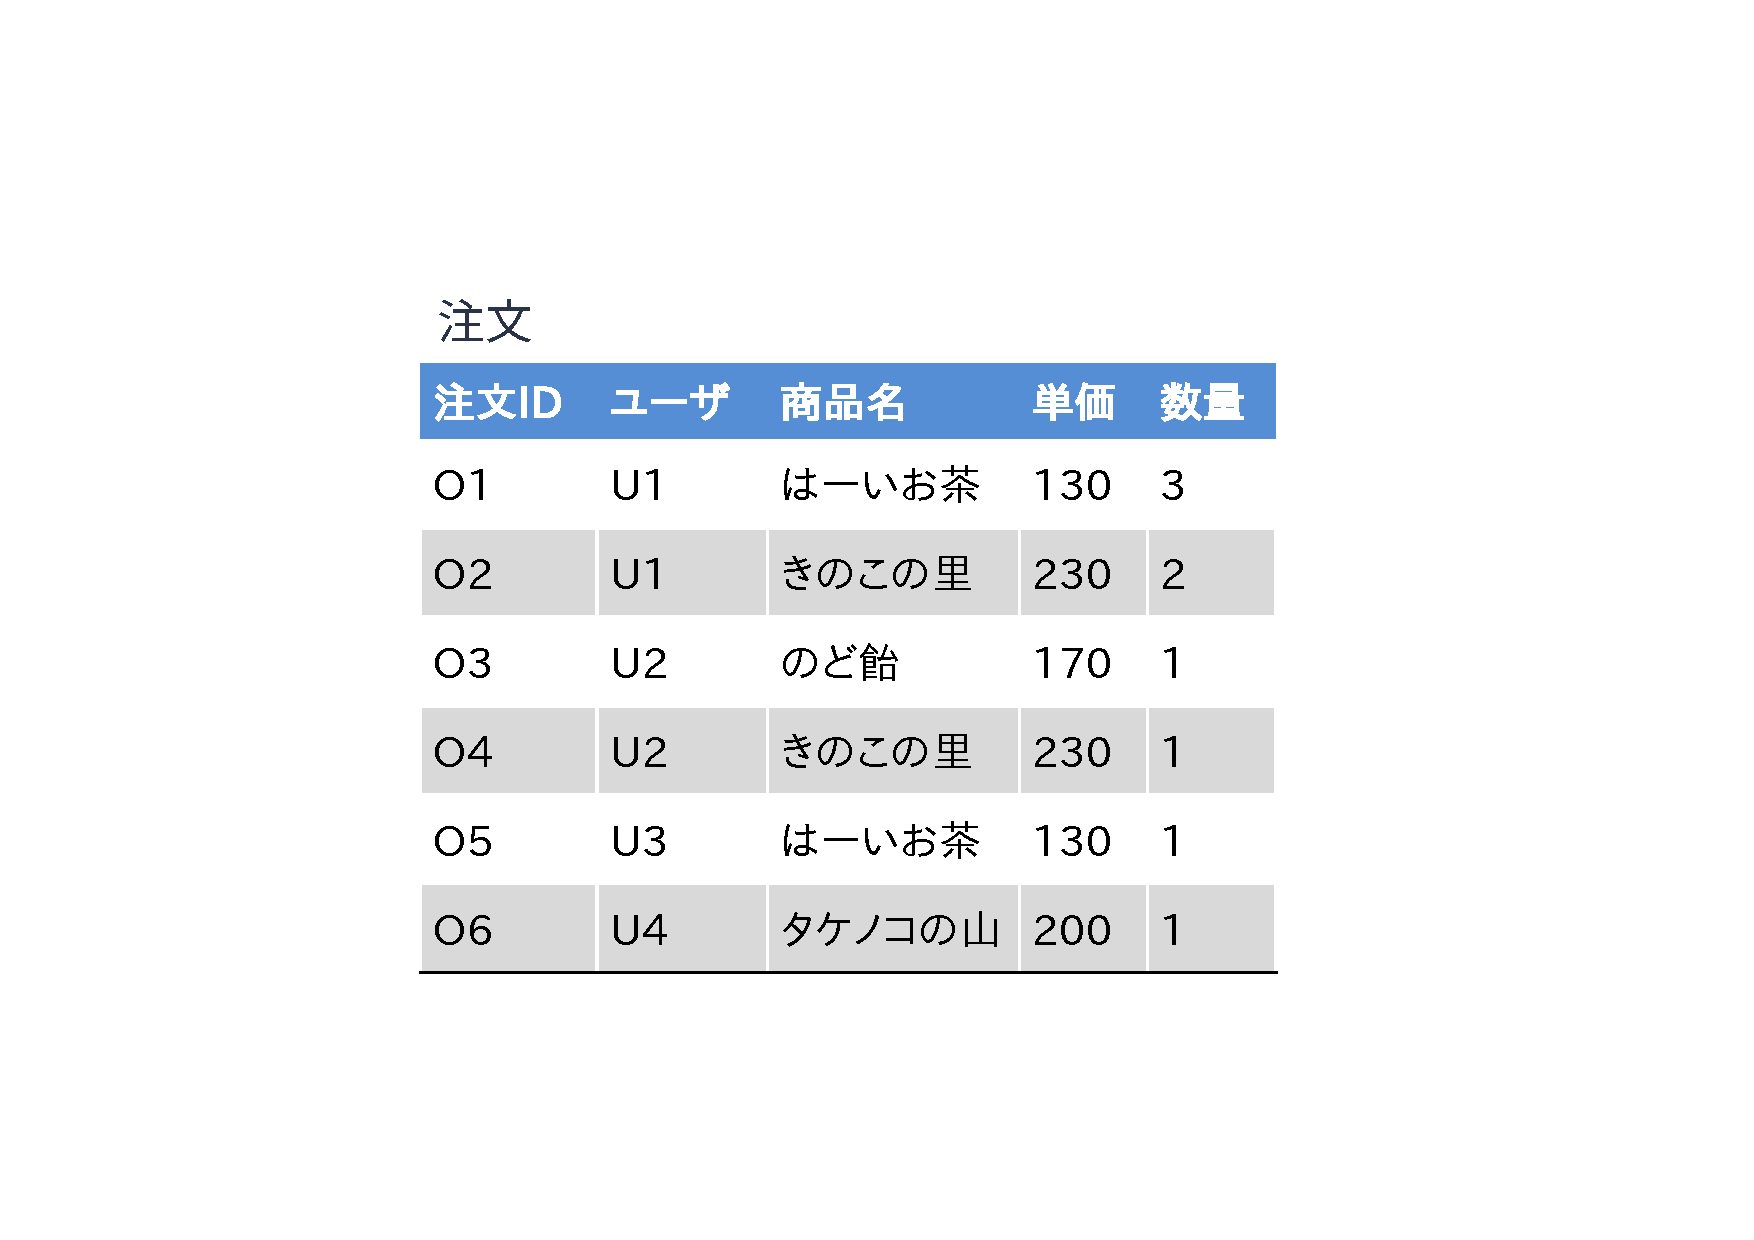
\includegraphics[width=0.7\textwidth]{figure/anomaly/order.pdf}
  \caption{ある時点までに蓄積された「注文」テーブル}
  \label{fig:order}
\endfigure

さて，山畑さんのショッピングサイトでは，新商品として\graybox{たきのこの里山}の取り扱いを開始することになりました．
新商品の情報をデータベースに登録するために，山畑さんは図\ref{fig:insertion-anomaly}のように「注文」テーブルに\graybox{(NULL, NULL, 'たきのこの里山', 250, NULL)}というレコードを追加しようとします．
ところが，RDBMSからデータの登録を拒否されてしまいました．
理由は，関係「注文」のスキーマにおいては\graybox{注文ID}が主キーとして設定されているからです．
まだ誰も注文していない\graybox{たきのこの里山}には\graybox{注文ID}が割り当てられていません．
そのため，主キーの値がないレコード\graybox{(NULL, NULL, 'たきのこの里山', 250, NULL)}はキー制約違反となって追加できないのです．
誰かが新商品を注文してくれないと新商品の情報をデータベースに登録できないとは，なんと不便なことでしょう．
山畑さんは「まだ誰も注文していない新商品」を登録できず，困ってしまいました…
\figure[tb]
  \centering
  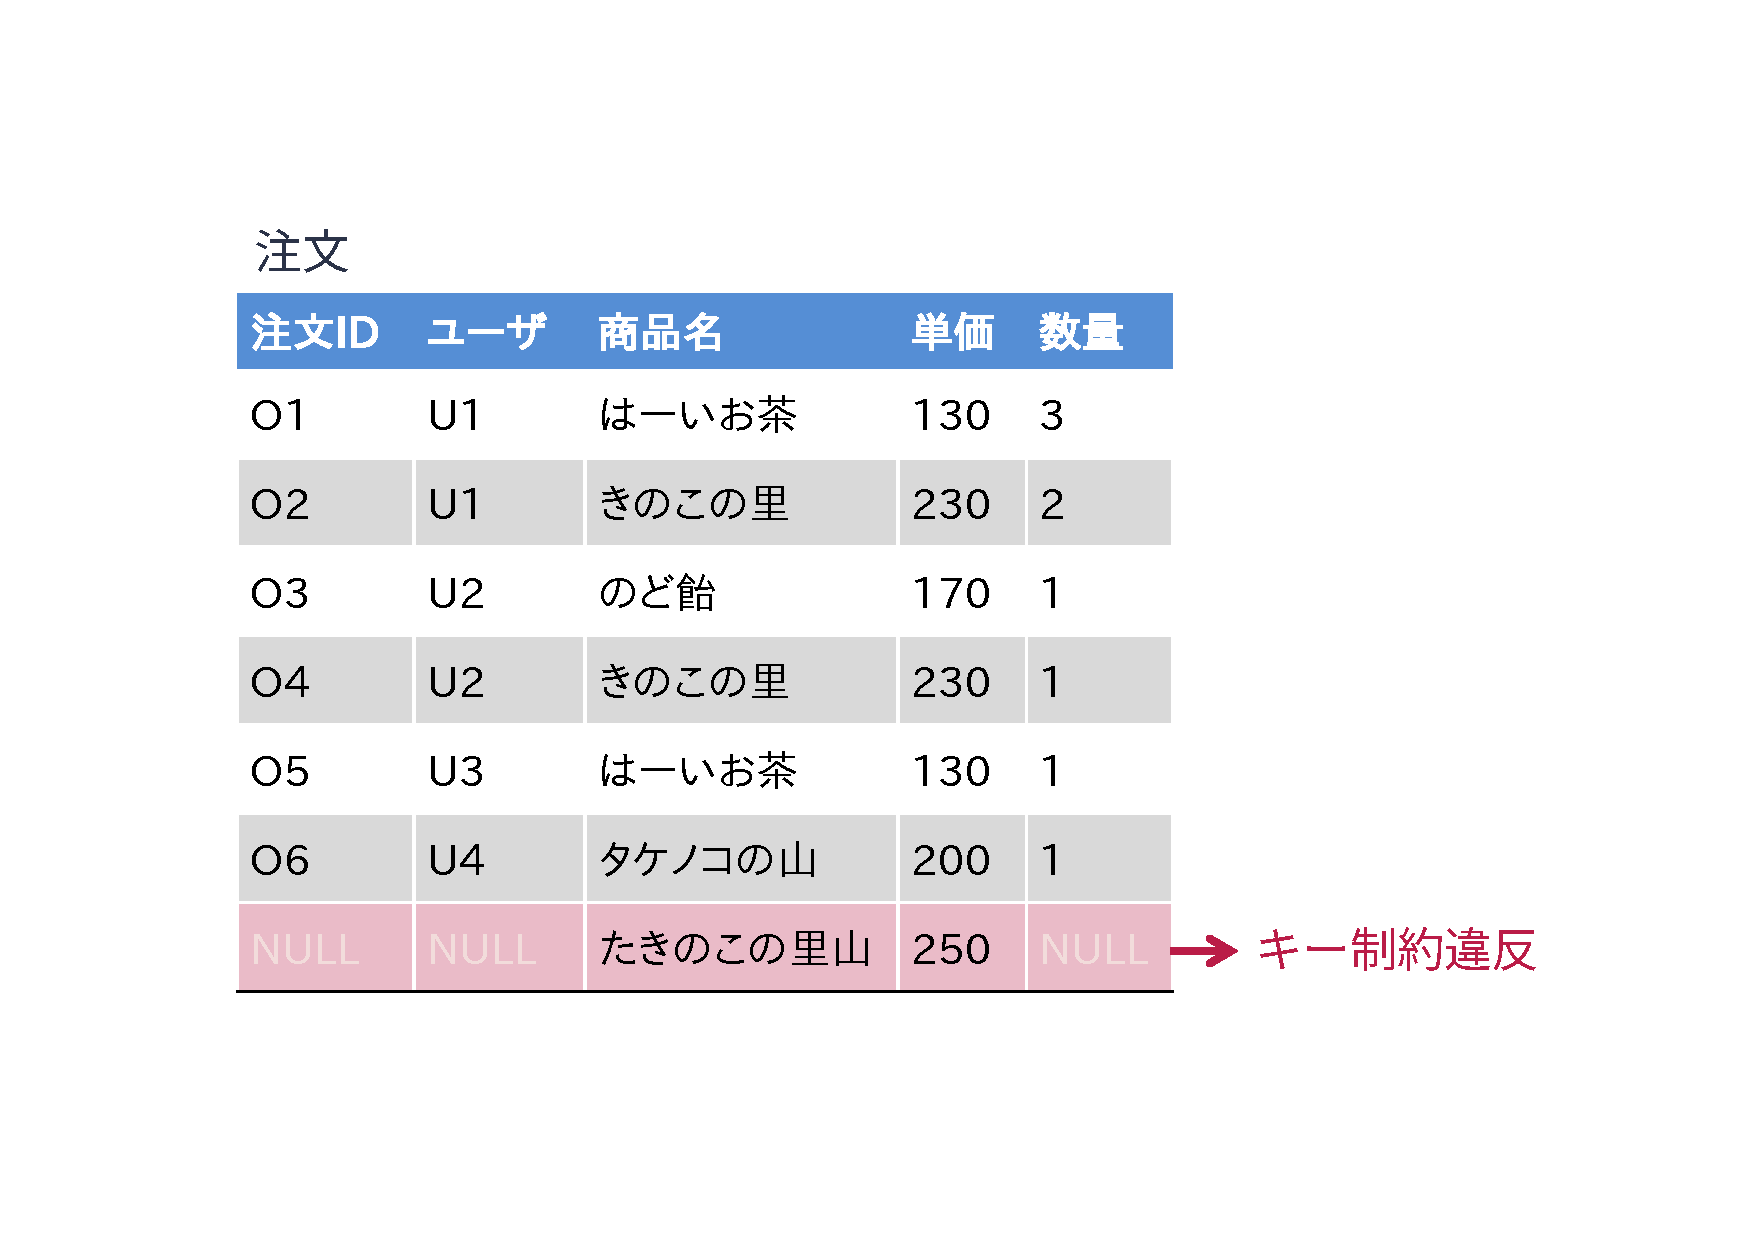
\includegraphics[width=0.9\textwidth]{figure/anomaly/insertion-anomaly.pdf}
  \caption{挿入時異状の例}
  \label{fig:insertion-anomaly}
\endfigure
このように，特定のレコードを挿入しようとしたときに，必要なデータが存在しないためにレコード登録ができない不都合な状態を\strong{挿入時異状（insertion anomaly）} と呼びます．



\section{削除時異状}
次に，図\ref{fig:order}のテーブルにおいて注文実績が1件しか存在しない\graybox{のど飴}について，ユーザ\graybox{U2}が払い戻しを希望したため，テーブルから関連する記録を削除しようとしているシーンについて考えてみましょう．
このとき，\strong{削除時異状（deletion anomaly）}と呼ばれる状態が発生します．

「注文」テーブルの設計の説明をした際，山畑さんはサイトで取り扱う商品についても「注文」テーブルの中で管理していると説明しました．
このような状況では，図\ref{fig:order}の3行目（注文IDが\graybox{O3}）のレコードを削除すると，図\ref{fig:deletion-anomaly}の状態になり，山畑さんのサイトで商品\graybox{のど飴}を取り扱っている事実や，商品の詳細情報（単価情報など）が意図しない形で失われてしまいます．
ユーザ\graybox{U2}は「注文をキャンセルしたかっただけ」なのに，サイト上は「\graybox{のど飴}という商品の存在そのものをデータベースから抹消してしまった」ことになります．
もし他のユーザが\graybox{のど飴}を買おうとしても，もうお店のサイトには並んでいない状態になってしまうのです．
このように削除時異状とは，あるレコードを削除したときに，残しておきたかった別の情報まで意図せずに消えてしまう状態を指します，
\figure[tb]
  \centering
  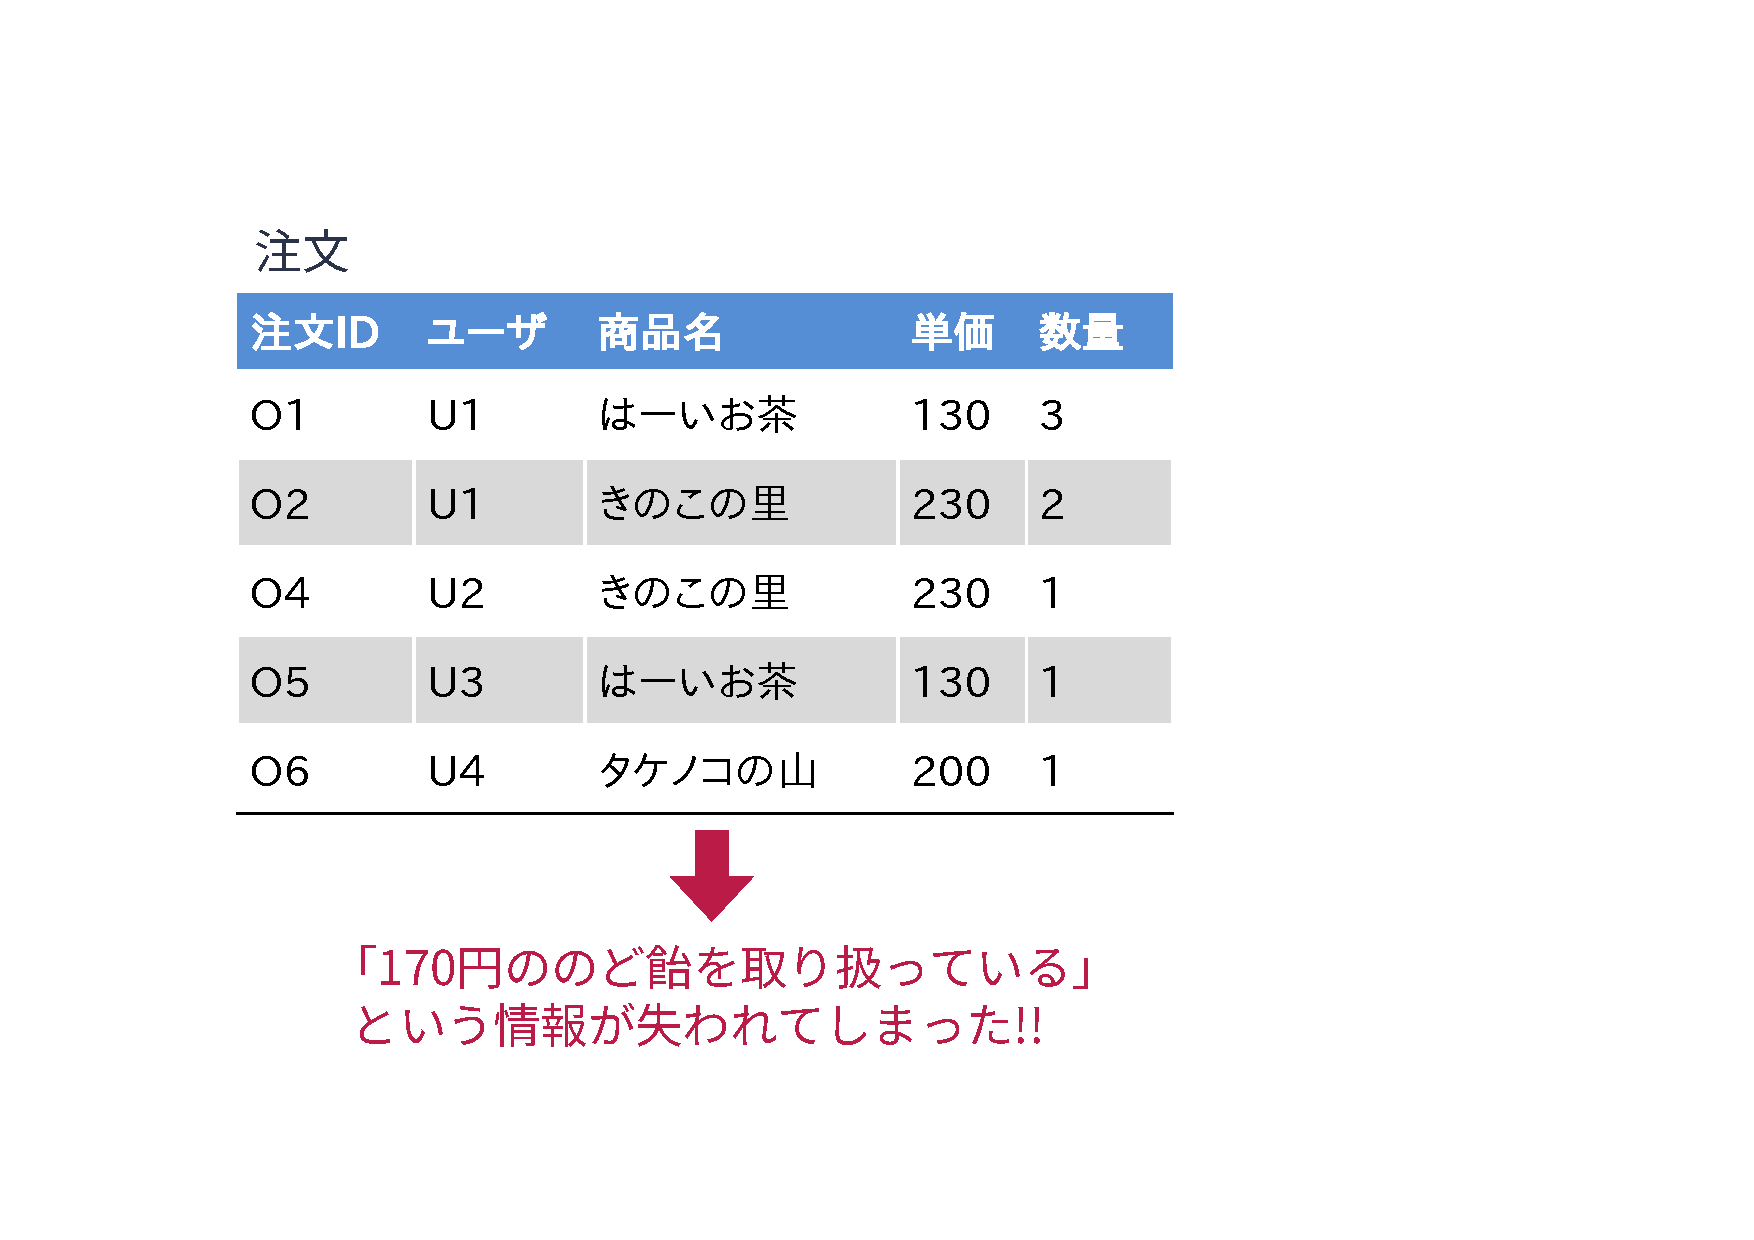
\includegraphics[width=0.8\textwidth]{figure/anomaly/deletion-anomaly.pdf}
  \caption{削除時異状の例}
  \label{fig:deletion-anomaly}
\endfigure

ところで，注文IDが\graybox{O3}のレコードを削除した後，山畑さんはのど飴の商品情報が消えてしまったことに気づいたとしましょう．
このとき，山畑さんが\graybox{(NULL, NULL, 'のど飴', 170, NULL)}というレコードを焦って追加して，\graybox{のど飴}の商品情報を復活させようとしても後の祭りです．
なぜなら，注文IDが存在しないため，このレコード追加しようとしても先に説明した挿入時異状が発生するからです．


\section{更新時異状}
3つ目の異状は\strong{更新時異状（update anomaly）}と呼ばれるものです．
例を見てみましょう．

図\ref{fig:order}のテーブルにおいて，\graybox{はーいお茶}の単価が\graybox{120円}であるにもかかわらず，山畑さんが勘違いして\graybox{130円}として注文テーブルに登録し続けていたとしましょう．
後日，山畑さんはこの誤りに気付きました．

さて，\graybox{はーいお茶}に関する注文は，注文IDが\graybox{O1}および\graybox{O5}の2件が該当します．
そのため，図\ref{fig:update-anomaly}のように，この2件の「単価」の値を\graybox{120}に書き換える必要があります．
ところが，山畑さんは該当商品の注文が1件しかないと思い込み，注文IDが\graybox{O1}のレコードの単価だけを修正し，\graybox{O5}の修正を忘れてしまいました．
ここで，山畑さんは「注文」テーブルの中でサイトの取扱商品も管理していたことを思い出してください．
先ほどのような修正忘れがあると，「注文」テーブルの中で同じ商品にも関わらず単価が異なる\graybox{はーいお茶}が存在することになり，どちらの単価が正しいのか分からない状態になってしまいます．
このように，一部のレコードの値を変更する際，更新漏れによるデータの矛盾が発生している状態を更新時異状と呼びます．
\figure[tb]
  \centering
  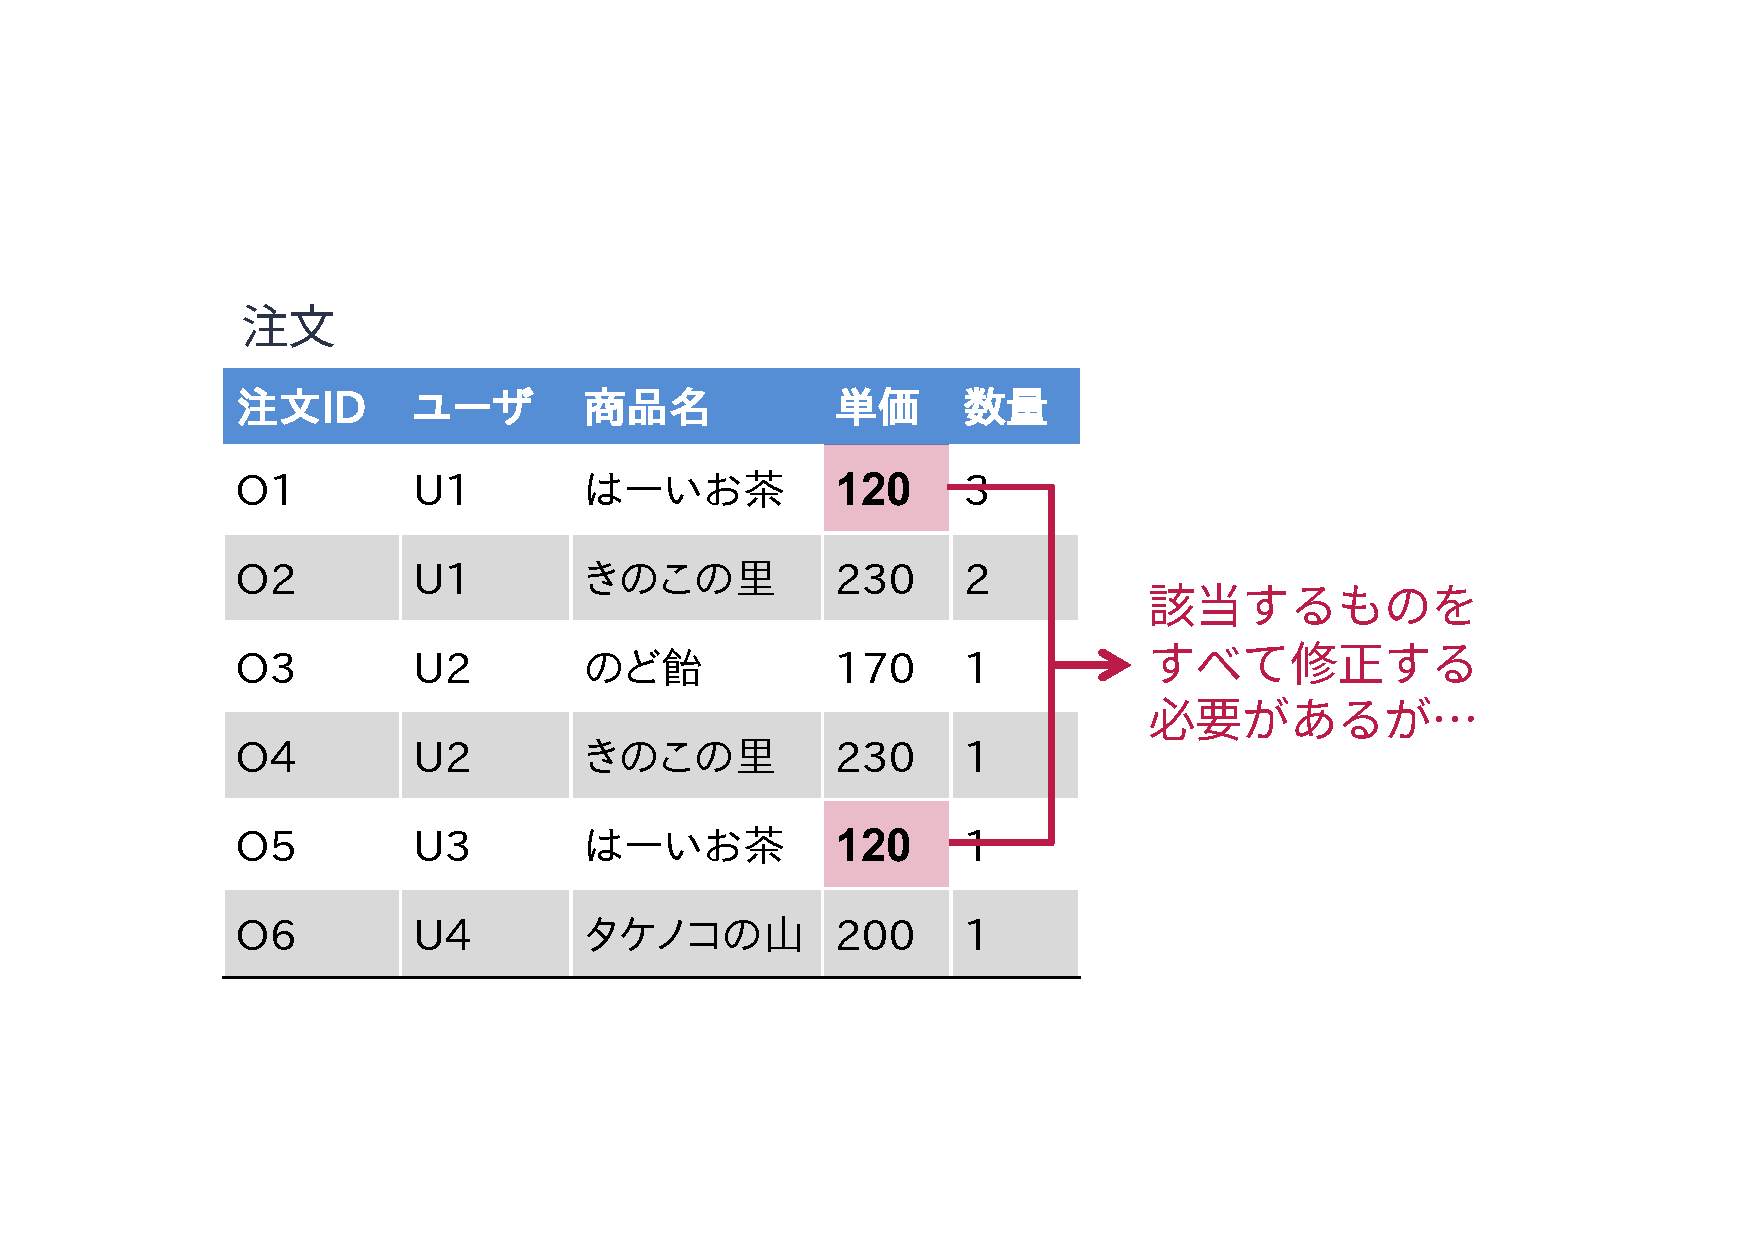
\includegraphics[width=0.9\textwidth]{figure/anomaly/update-anomaly.pdf}
  \caption{更新時異状の例}
  \label{fig:update-anomaly}
\endfigure

今回の例では「はーいお茶の単価が120円の間違いだった」という単一の商品に関する修正事象にもかかわらず，データベース上では2件のレコードの書き換え（修正）の必要がありました．
図\ref{fig:update-anomaly}の例では\graybox{はーいお茶}の注文履歴が2件しかありませんでしたが，修正対象となる履歴が100万件あれば100万回の修正が必要になります．
このように，データの重複が多いという状態は\strong{冗長性が高い}と表現されます．
データベースの冗長性が高いと，修正漏れが発生する可能性が高まるだけでなく，修正作業自体も非常に大変なものになってしまいます．


\section{異状を防ぐには}
上記のような「挿入時異状」「削除時異状」「更新時異状」が起きないようにするには，どうしたらよいのでしょうか．
\begin{itemize}
  \item 「注文」テーブルの中で商品情報も管理しているのが間違いなのでは…
  \item \ref{chap:sql-part1}章の説明で出てきた「商品」テーブルのように，商品の詳細情報を管理するためだけのテーブルを作ったら良いのでは…
\end{itemize}
このように考えた方は鋭いです．

山畑さんの「注文」テーブルの問題は，商品に関する属性を注文履歴と分けて扱えるにも関わらず，両者を同じテーブルの中で詰め込んで管理していることが原因でした．
山畑さんの異状問題を解決するためには，図\ref{fig:decomposition-example}のように，「注文」テーブルから商品に関する属性を切り離して，注文履歴とは別に商品情報を管理するための「商品」テーブルを作っておけばよかったのです．
このようにすれば，新商品である「たきのこの里山」を取り扱い商品に追加したい場合は，「商品」テーブルにそれに関するレコードを追加するだけで済み，挿入時異状が発生しません．
また，注文IDが\graybox{O3}のレコードを削除しても，「商品」テーブルの中の「のど飴」のレコードは残るため，削除時異状も発生しません．
「はーいお茶」の価格を変更する必要が生じても，「商品」テーブルの中の「はーいお茶」のレコードの「価格」を1箇所書き換えるだけで済むため，更新時異状も発生しません．
「注文」テーブルには商品の単価情報がありませんが，必要なときは「商品」テーブルを参照すれば，該当する商品の単価を知ることができます．
\figure[tb]
  \centering
  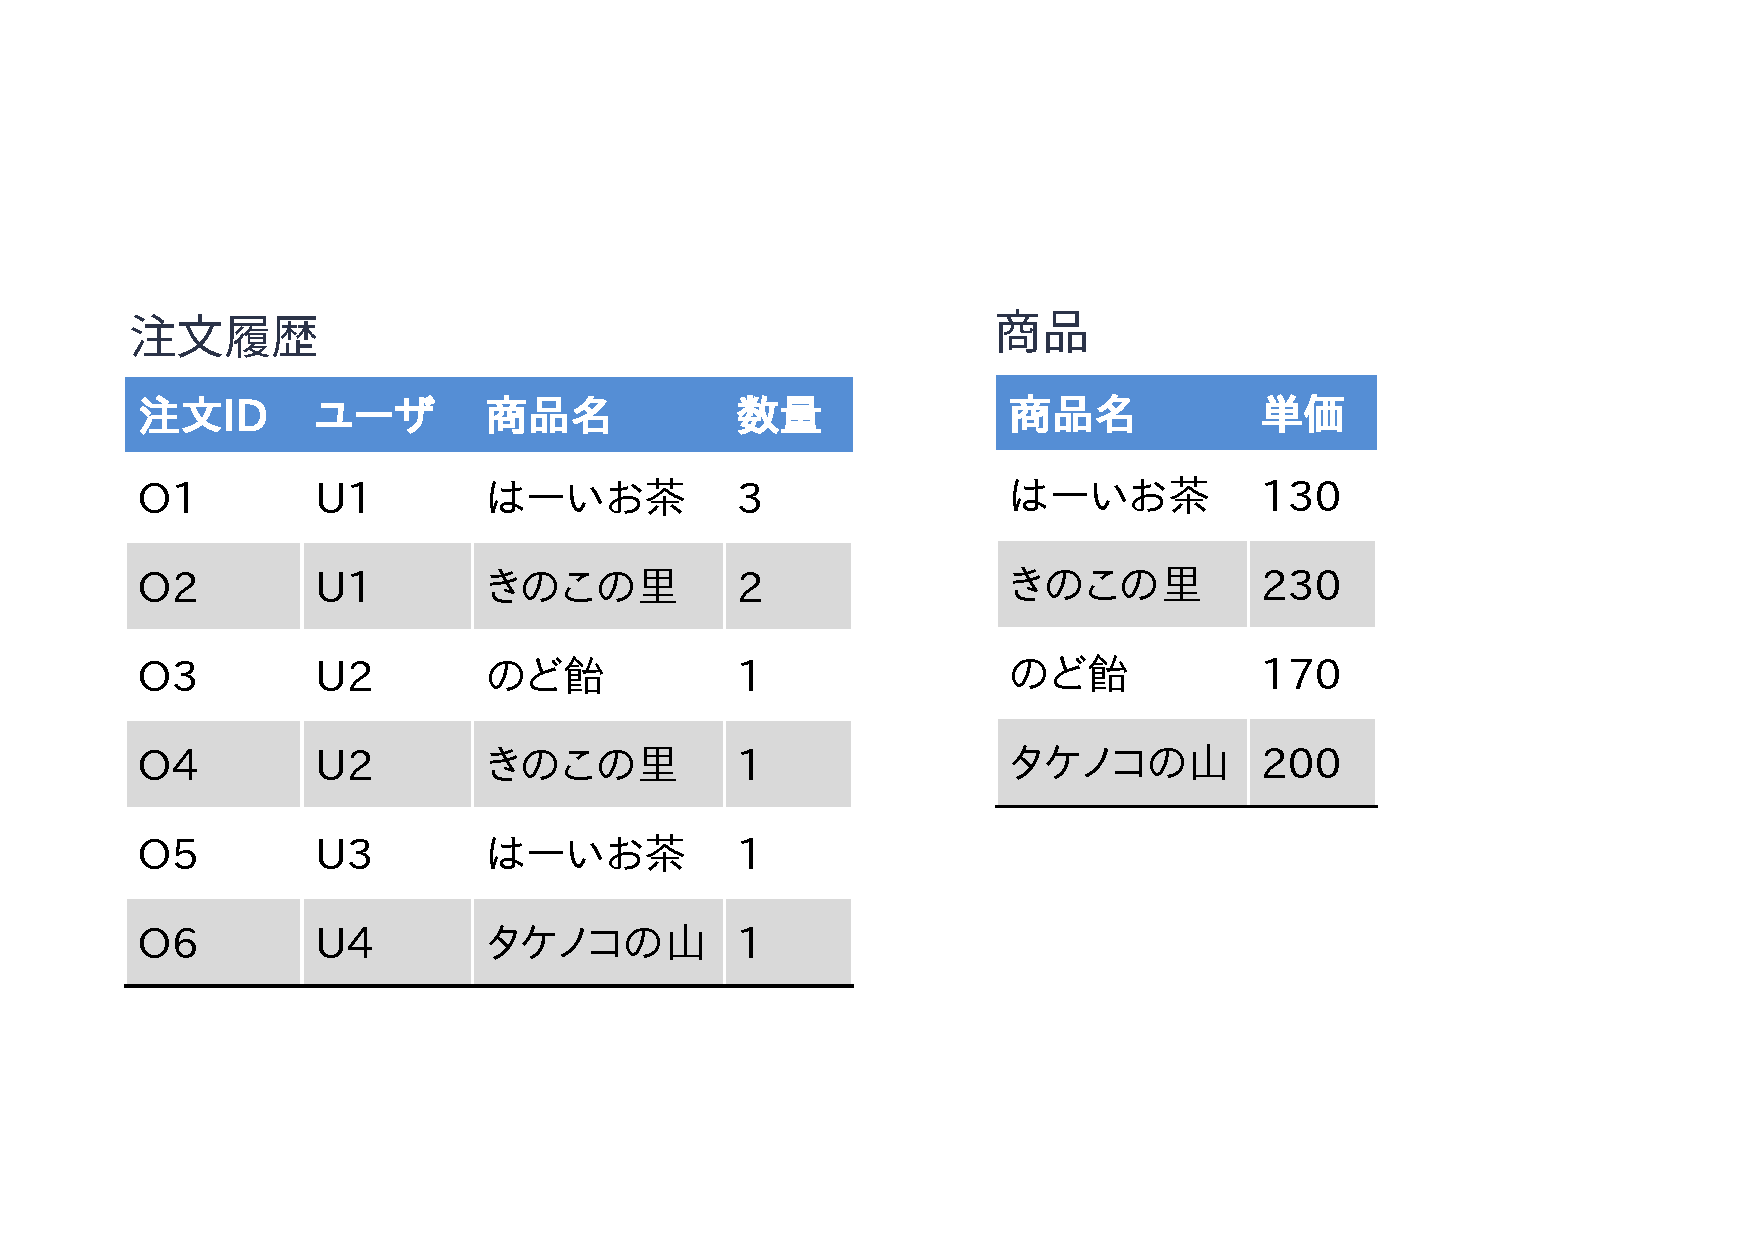
\includegraphics[width=0.9\textwidth]{figure/anomaly/decomposition-example.pdf}
  \caption{「注文」テーブルから商品に関する属性を切り離して「商品」テーブルを作ることによって異状を防ぐ例}
  \label{fig:decomposition-example}
\endfigure

このように，データベースの異状は関係スキーマ（テーブルの構造）を適切に設計することによって防ぐことができます\cite{Bernstein1976}．
今回の例では「注文」テーブルから商品に関する情報を切り出して「商品」テーブルを作ればよいということが直感的に分かりました．
しかし，実際のデータベースの設計においてはデータ間の関係が複雑であることも多く，テーブルの中で取り扱うべき属性情報を決めるのも簡単なことではありません．
そこで次章では，データを正しく矛盾なく保つための適切な関係スキーマの設計方法について学びましょう．


% ---------------------------------------
%\hrulefill
\section{クイズ}
% ---------------------------------------
\subsubsection{Q1. 異状の分類}
ある大学の授業システム上で，以下のような「履修登録」テーブルが作られました．
主キーは\graybox{\{学生ID, 科目ID}\}です．

\begin{equation*}
  \text{履修登録}(\underline{\text{学生ID, 科目ID}}, \text{学生名}, \text{科目名}, \text{担当教員})
\end{equation*}

このテーブルを運用していたところ，以下の(1)〜(3)のトラブルが発生しました．
それぞれ，「挿入時異状」「削除時異状」「更新時異状」のどれに該当するか答えなさい．
\begin{enumerate}
\item 科目「データサイエンス入門」が新設され，担当教員も決まったが，まだ誰も履修登録をしていないため，データベースに科目を登録できない．

\item「プログラミング基礎」という科目を担当していた教員が変わったため，この科目を履修している学生100人分のレコードすべての「担当教員」を書き換えなければならず，一部で修正漏れが発生した．

\item 「離散数学」という科目を履修していた唯一の学生が履修を取り消した（レコードを削除した）ところ，「離散数学」という科目が存在したこと，誰が担当教員だったのかという情報までデータベースから消えてしまった．
\end{enumerate}


\subsubsection{Q2. 更新時異状}
架空の家具販売店「八高家具」では顧客と購入希望商品の「ペア」（誰が何の商品の購入を希望しているか）で営業担当を割り当てています．
営業担当は年度ごとに営業成績が評価されることになっています．

八高家具では，下記関係スキーマに従った関係データモデルを用いて営業記録，取扱商品，営業成績の管理を行っています．
\begin{equation*}
  \text{営業記録}(\underline{\text{ユーザ}}, \text{商品}, \text{連絡先}, \text{メーカー}, \text{営業担当}, \text{営業成績})
\end{equation*}

図\ref{fig:sale-history}は，関係スキーマ「営業記録」にしたがって八高家具における営業記録を記録したテーブルです．
営業担当者の成績の修正に際して，関係「営業記録」のみを用いてデータを管理する際に発生しうる更新時異状の例を挙げなさい．
\figure[htb]
  \centering
  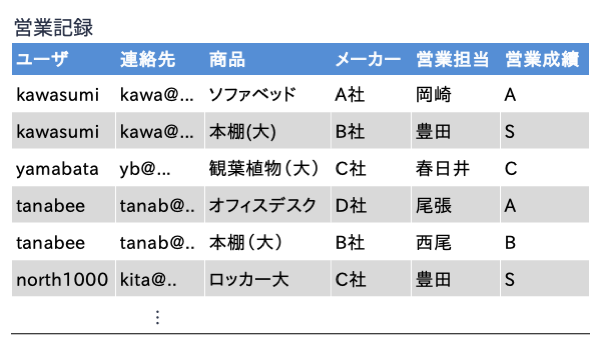
\includegraphics[width=0.7\textwidth]{figure/anomaly/sale-history.png}
  \caption{八高家具の「営業記録」テーブル}
  \label{fig:sale-history}
\endfigure


\subsubsection{Q3. 削除時異状}
架空の家具販売店「八高家具」では，以下のような修正した関係スキーマを用いて，改めて営業記録をつけ始めました．
\begin{equation*}
  \text{営業記録2}(\underline{\text{ユーザ}, \text{商品}}, \text{連絡先}, \text{メーカー}, \text{営業担当})
\end{equation*}

図\ref{fig:sale-history2}は，関係スキーマ「営業記録2」にしたがって営業記録を記録したテーブルです．
営業担当者の成績の修正に際して，関係「営業記録2」のみを用いてデータを管理する際に発生しうる削除時異状の例を挙げなさい．
\figure[htb]
  \centering
  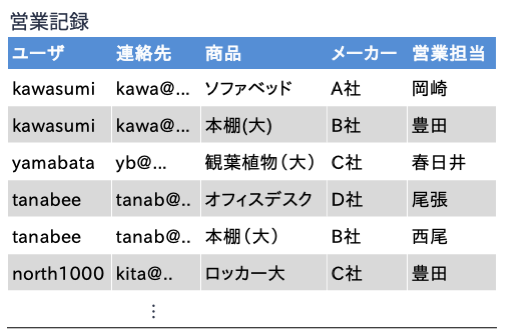
\includegraphics[width=0.7\textwidth]{figure/anomaly/sale-history2.png}
  \caption{八高家具の「営業記録2」テーブル}
  \label{fig:sale-history2}
\endfigure


\subsubsection{Q4. 挿入時異状}
架空の家具販売店「八高家具」では，更に修正した以下の関係スキーマを用いて改めて営業記録をつけ始めました．
\begin{equation*}
  \text{営業記録3}(\underline{\text{ユーザ}, \text{商品}},  \text{メーカー}, \text{営業担当})
\end{equation*}

図\ref{fig:sale-history3}は，関係スキーマ「営業記録3」にしたがって営業記録を記録したテーブルです．
営業担当者の成績の修正に際して，関係「営業記録3」のみを用いてデータを管理する際に発生しうる挿入時異状の例を挙げなさい．
\figure[htb]
  \centering
  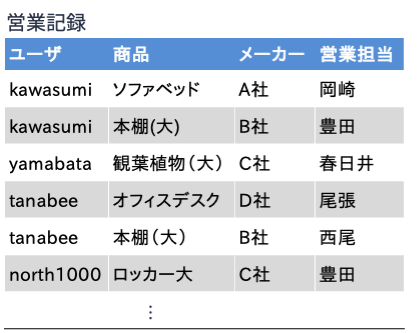
\includegraphics[width=0.7\textwidth]{figure/anomaly/sale-history3.png}
  \caption{八高家具の「営業記録3」テーブル}
  \label{fig:sale-history3}
\endfigure


